% !TeX root = ../main.tex

\chapter{Physics of semiconductors}

\section{Intrinsic semiconductors}

The number of particles
\begin{equation}
  n = \int_{E_c}^\infty \d E g(E) f(E)
\end{equation}
where
\[
  g(E) = \frac{m_n^*}{\pi^2\hbar^3} \sqrt{2m_n^*(E - E_c)}
\]
Typically, $E_f$ is inside the band gap.
In most cases, the energy $E \gg E_f$.
So, the distribution function is
\[
  f(E) = \frac1{\upe^{(E-E_f)/kT} + 1} \approx \upe^{-(E-E_f)/kT}
\]
Then, the integral
\begin{equation}
  n = \int_{E_c}^\infty \frac{m^*}{\pi^2\hbar^3} \sqrt{2m^*(E - E_c)}
      \upe^{-(E-E_f)/kT} \d E = N_c\upe^{-(E_c-E_f)/kT}
\end{equation}
where $N_c = \frac{2(2\pi m_e^* kT)^{3/2}}{h^3}$.

One can simplify understanding the density of carrier is proportional to
\begin{equation}
  n_i^2 = n \cdot p = N_c \cdot N_v \upe^{-E_k/kT}
\end{equation}
$n$ and $p$ satisfies
\[
  \begin{cases}
    n + N_a & = p + N_d,\\
    np & = n_i^2
  \end{cases}
\]
then, we can solve
\begin{align}
  n & = \frac{N_d - N_a}{2} + \ab[\ab(\frac{N_d - N_a}{2})^2 + n_i^2]^2,\\
  p & = \frac{N_a - N_d}{2} + \ab[\ab(\frac{N_a - N_d}{2})^2 + n_i^2]^2,
\end{align}
\begin{enumext}[wrap-label = \underline{Case #1}, label = \arabic*,
                      list-indent = 0pt]
  \item $n$-type: $N_d - N_a \gg n_i$
  \item $p$-type: $N_d - N_a \ll n_i$
\end{enumext}
This p-n junction is consist with p-dropped and n-dropped silicon
\begin{center}
  \begin{minipage}{.48\linewidth}
    \centering
    p-side\par
    \begin{tikzpicture}
    \draw (0,0) node [left] {$E_v$} --++ (2,0);
    \draw[dashed] (0,.5) node [left] {$E_f$} --++ (2,0);
    \draw (0,1.5) node [left] {$E_c$} --++ (2,0);
  \end{tikzpicture}
  \end{minipage}
  \hspace* \fill
  \begin{minipage}{.48\linewidth}
    \centering
    n-side\par
    \begin{tikzpicture}
    \draw (0,0) --++ (2,0) node [right] {$E_v$};
    \draw[dashed] (0,1) --++ (2,0) node [right] {$E_f$};
    \draw (0,1.5) --++ (2,0) node [right] {$E_c$};
  \end{tikzpicture}
  \end{minipage}
\end{center}
The homojunction: have the same band gap and abnd element.

\paragraph{Behavior of $\mathsf{V}$}

If apply a positive voltage $V$, then, build-in potential will reduce;
If apply a negative voltage $V$, then, build-in potential will increase.

\paragraph{Semiconductor heterstructure}

Connect two different semiconductors together, and the bandgap can be different,
also, the band alignment can be different.
\begin{enumext}
  \item Type I: straddling gap. Application: 2DEG
  \begin{center}
    \begin{tikzpicture}
      \draw (0,0) node [left] {$E_C$} -- (1,0) --
            (1,.5) -- (2,.5) -- (2,0) -- (3,0);
      \draw (0,2) node [left] {$E_V$} -- (1,2) --
            (1,1.5) -- (2,1.5) -- (2,2) -- (3,2);
    \end{tikzpicture}
  \end{center}
  The generation is \ce{AlGaAs}, which provide the carier $n$,
  and the conducting channel is \ce{GaAs}, which untdout dopes.
  \item Type II: staggered gap.
  
  For electrons, the electrons locate in layer 2, but for holes, it locate in
  layer 1, they are separated. They can interact with each other by Coulomb
  interaction.
  \begin{center}
    \begin{minipage}{.48\linewidth}
      \centering
      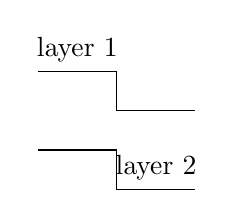
\begin{tikzpicture}
      \draw (0,0) -- (1,0) -- (1,-.5) -- node [above] {layer 2} (2,-.5);
      \draw (0,1) -- node [above] {layer 1} (1,1) -- (1,.5) -- (2,.5);
    \end{tikzpicture}
    \end{minipage}
    \begin{minipage}{.48\linewidth}
      \centering
      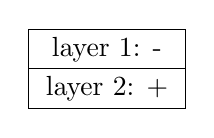
\begin{tikzpicture}
      \draw (0,0) rectangle (2,.5) node [midway] {layer 2: +};
      \draw (0,.5) rectangle (2,1) node [midway] {layer 1: -};
    \end{tikzpicture}
    \end{minipage}
  \end{center}
  Without combinations, they can have a longer lifetime.
  \item Type III: broken gap.
\end{enumext}